%! Author = Gianni
%! Date = 08/02/2024

\chapter{Home Assistant}
\label{ch:homeassistant}

\section{Implementazione nel progetto}
\label{sec:hass-introduzione}
Home Assistant è un software open-source e gratuito per la domotica, 
progettato per essere una piattaforma di integrazione indipendente dall'ecosistema dell'Internet of Things (IoT) 
e un sistema di controllo centrale per i dispositivi smart, 
con particolare attenzione al controllo locale e alla privacy.
Permette di raccogliere i dati provenienti da diversi sensori e di mostrarli in un'interfaccia grafica.
Nel progetto questo software era già installato in una macchina, 
per i dettagli sull'installazione si rimanda alla documentazione ufficiale \cite{hass-installazione}. 
Si doveva solo procedere con la configurazione per ricevere i dati da vari topic del Broker MQTT 
e mostrare i valori in un'interfaccia apposita.
Tuttavia prima viene spiegata una modifica che si è dovuto fare per risolvere un problema con i 
servizi di auto-discovery del software.

\section{Servizi di auto-discovery}
\label{sec:hass-servizi}
Home Assistant fornisce vari servizi tra cui quelli di auto-discovery.
Questi permettono di scoprire nella rete LAN a cui si è connessi le possibili sorgenti dati da integrare nel sistema.
Tuttavia dato che Home Assistant era installato all'interno della rete universitaria,
questi servizi creavano moltissime richieste a causa dell'elevato numero di dispositivi presenti.
È quindi stato necessario modificare la configurazione per disabilitare l'auto-discovery.
La configurazione di Home Assistant si trova all'interno del file configuration.yaml.
Questo file in base al tipo di installazione eseguita può essere modificato da interfaccia grafica o
da riga di comando.
Nel nostro caso l'installazione è stata fatta tramite container Docker, 
quindi il file di configurazione era modificabile da riga di comando e si trovava nella seguente cartella:
\begin{lstlisting}[language=textnonum]
    /var/docker
\end{lstlisting}
Nel file è presente di default la seguente configurazione:
\begin{lstlisting}[language=textnonum]
    default_config:
\end{lstlisting}
Con questa configurazione si abilitano usa serie di componenti che di solito sono utili per semplificare l'uso
del software, tra cui quelli di auto-discovery.
Per risolvere il problema è stata commentata quella configurazione 
e sono state aggiunte tutte le configurazioni a cui corrispondeva disabilitando quelle di auto-discovery.
In base alla versione di Home Assistant, 
la configurazione può corrispondere a un numero maggiore o minore di servizi.
In questa installazione era presente la versione 2023.3.1 
e quel parametro corrispondeva ai seguenti servizi:
\begin{lstlisting}[language=bash]
    #automation: !include automations.yaml ALREADY PRESENT 
    backup:
    bluetooth:
    #cloud:
    config:
    counter:
    #dhcp:
    energy:
    #frontend: ALREADY PRESENT 
    hardware:
    history:
    homeassistant_alerts:
    image:
    input_boolean:
    input_button:
    input_datetime:
    input_number:
    input_select:
    input_text:
    logbook:
    map:
    media_source:
    mobile_app:
    my:
    #network:
    person:
    schedule:
    #scene: !include scenes.yaml ALREADY PRESENT 
    #script: !include scripts.yaml ALREADY PRESENT 
    #ssdp:
    #stream:
    sun:
    system_health:
    tag:
    timer:
    usb:
    webhook:
    #zeroconf:
    zone:
\end{lstlisting}
I parametri che hanno un cancelletto davanti sono disattivati.
I parametri seguiti da ALREADY PRESENT 
sono stati attivati in modo diverso da un'altra parte nel file della configurazione.
I parametri importanti da disattivare erano cloud, dhcp, network, ssdp, stream e zeroconf.
In questo modo sono stati disabilitato completamente i servizi di auto-discovery 
e sono state ridotte al minimo le richieste che Home Assistant eseguiva nella rete.
Si rimanda alla documentazione per sapere il significato di ogni parametro \cite{hass-config}.
Nella community di Home Assistant ci sono state altre persone 
che hanno dovuto affrontare lo stesso problema, 
riporto alcuni casi che mi sono stati utili \cite{hass-config-community1} \cite{hass-config-comumnity2}.

\section{Integrazione con MQTT}
\label{sec:hass-MQTT}
Per far ricevere a Home Assistant i messaggi del broker MQTT si devono fare due passaggi.
Il primo è configurare il client per connettersi al broker 
e il secondo è definire un sensore per ogni valore presente nel messaggio in arrivo dal Broker.
Per configurare il client si deve eseguire la procedura da interfaccia web, 
come spiegato nella documentazione \cite{hass-mqtt}.
Quindi per inserire la configurazione si deve andare in "Impostazioni", poi "dispositivi e servizi",
premere in basso a destra il pulsante + e selezionare dalla lista "MQTT".
A questo punto si apre una finestra che deve essere popolata con la configurazione per la connessione
come se fosse un normale client MQTT.
La configurazione usata nel progetto è la seguente:
\begin{lstlisting}[language=textnonum]
    broker: mydomain.it
    port: 8883
    username: username
    password: password
    client ID: (vuoto)
    time: (60 il valore di default)
    Usa un certificato client: False
    Convalida del certificato: automatico
    Ignora la convalida del certificato del broker: True
    Protocollo MQTT: 3.1.1
    Trasporto MQTT: TCP
\end{lstlisting}
Poi si preme su avanti e si segue le richieste fino a completare la procedura.
Si è quindi configurato il client che riceve i messaggi.
Home Assistant supporta la configurazione di un broker alla volta.
Nel secondo passaggio si deve modificare il file configuration.yaml per aggiungere i vari sensori.
Nel file si deve aggiungere ad esempio il seguente codice:
\begin{lstlisting}[language=bash]
    mqtt:
        sensor:
            - name: Serra reale Temperatura Aria
              state_topic: sensori
              unique_id: sensor.reali.serraAirTemperature
              unit_of_measurement: "°C"
              value_template: >
              
                  {{ value_json.Temp__C }}
              
                  {{ sensor.reali.serraAirTemperature }}
              
\end{lstlisting}
La prima riga indica che il sensore che si sta aggiungendo ha come sorgente il broker MQTT.
Poi nella seconda lista si specifica di che tipo è il sensore, 
in questo caso è indicato un semplice sensore.
Poi si definisce il sensore iniziando la dichiarazione con "- ".
Viene indicato il nome visualizzato nell'interfaccia grafica, il topic da cui prendere il messaggio,
un id unico per identificare il sensore, 
l'unità di misura e infine come il valore deve essere visualizzato.
Nel campo valore è possibile definire la logica per eseguire controlli, modifiche o altro 
per ottenere il valore finale.
Per aggiungere altri sensori, basta inserire altre definizioni prestando attenzione all'indentazione
e ricordandosi di mettere "- " prima della definizione.
Nell'appendice vengono riportati altri esempi di definizioni di sensori~\ref{sec:hass-appendix-sensori}.

\section{Visualizzazione dei dati}
\label{sec:hass-visualizzazione}
Per configurare come vengono visualizzati i dati, si deve agire da interfaccia grafica.
Come prima cosa si deve creare una nuova plancia (in inglese dashboard).
Si deve andare in "Impostazioni", poi "Plance" e in basso a sinistra premere su +.
Si apre una finestra in cui si deve mettere il nome della plancia, un'icona, l'URL e altre impostazioni.
Una volta configurato, si preme su crea e nella barra a sinistra si aggiungerà la nuova plancia.
Successivamente si può iniziare a configurare la visualizzazione,
si consiglia di guardare la documentazione per tutte le possibilità di personalizzazione \cite{hass-dashboard}.
Si va nella plancia appena creata, in alto a destra si apre il menù e si seleziona "modifica plancia".
Poi si clicca di nuovo sul menù in alto a destra e si seleziona "Editor di configurazione testuale".
Viene visualizzato un file simile a quello di configurazione.
Di seguito viene riportata una parte della configurazione di una plancia:
\begin{lstlisting}[language=bash]
    title: Oidio
    background: center / cover no-repeat fixed url('/local/background_verde_sfumature.jpg')
    views:
      - theme: Backend-selected
        title: Normale
        icon: ''
        path: normale
        badges: []
        cards:
          - type: vertical-stack
            cards:
              - type: entities
                title: Riepilogo Sensori
                entities:
                  - entity: sensor.serra_reale_temperatura_aria
                    name: Temperatura Aria
          - type: vertical-stack
            cards:
              - type: picture-elements
                title: Stime Rischio Oidio
                image: http://mydomain.it:8123/local/Mappa_new.png
                elements:
                  - type: state-badge
                    entity: sensor.serra_stima_oidio_rischio_1
                    style:
                      top: 28%
                      left: 37%
                      scale: 90%
                      color: rgba(0,0,0,0)
\end{lstlisting}
Nella configurazione alla prima riga c'è il nome della plancia.
La seconda riga definisce il background che deve avere la plancia.
L'immagine è salvata in una cartella accessibile da Home Assistant che è 
\begin{lstlisting}[language=textnonum]
    /var/docker/www
\end{lstlisting}
Poi viene definita una scheda della plancia con il tema, il titolo, nessuna icona e il path dell'URL.
Poi si definiscono le cards, che sono i gruppi di elementi che devono essere mostrati.
Il primo gruppo viene definito come un insieme di card verticali.
Al suo interno c'è una card che contiene entità e ha nome "Riepilogo sensori".
Le entità in questo caso sono solo una: un sensore identificato da un nome univoco e il nome visualizzato.
Anche il secondo gruppo è un insieme di card verticali.
Contiene una card di tipo immagine-elementi che permette di visualizzare un'immagine 
con sopra i valori dei sensori.
Viene impostato il titolo, l'immagine in background e la lista di elementi.
L'immagine è sempre contenuta nella cartella del background.
Gli elementi in questo caso sono solo uno, che è di tipo badge.
Viene specificato il nome univoco del sensore da cui prendere i dati
e vengono definiti degli stili del badge.
Nell'appendice vengono riportate le definizioni usate~\ref{sec:hass-appendix-plancia}.
Una volta terminata l'impostazione delle varie card e delle relative sorgenti, 
si preme "salva" in alto a destra e poi su "fatto".
In questo modo si è ottenuta la visualizzazione di due sensori con sorgente MQTT modificando la plancia.\newline
Di seguito viene riportata l'immagine di uno dei risultati che è stato raggiunto 
modificando opportunamente questo file.

\begin{figure}[htp]
    \centering
    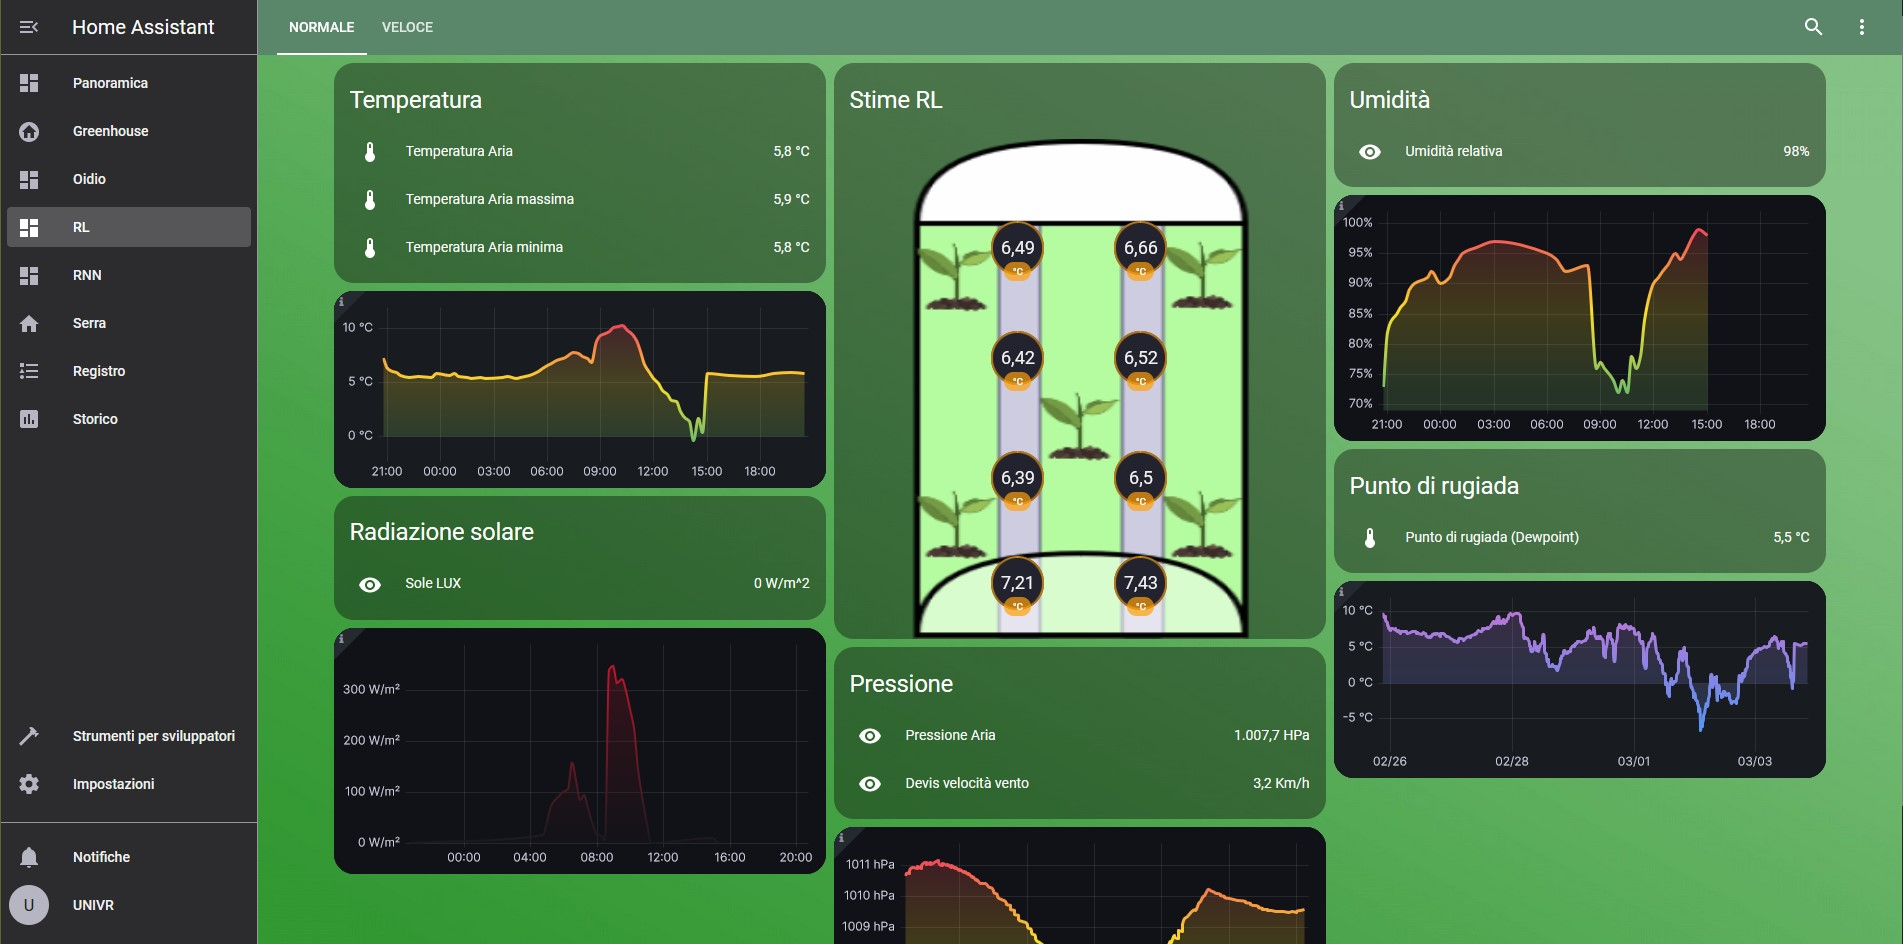
\includegraphics[width=1\linewidth]{images/chapter5-hass-visualizzazione.jpg}
    \caption{Plancia RL}
\end{figure}